%% bare_jrnl.tex
%% V1.4a
%% 2014/09/17
%% by Michael Shell
%% see http://www.michaelshell.org/
%% for current contact information.
%%
%% This is a skeleton file demonstrating the use of IEEEtran.cls
%% (requires IEEEtran.cls version 1.8a or later) with an IEEE
%% journal paper.
%%
%% Support sites:
%% http://www.michaelshell.org/tex/ieeetran/
%% http://www.ctan.org/tex-archive/macros/latex/contrib/IEEEtran/
%% and
%% http://www.ieee.org/

%%*************************************************************************
%% Legal Notice:
%% This code is offered as-is without any warranty either expressed or
%% implied; without even the implied warranty of MERCHANTABILITY or
%% FITNESS FOR A PARTICULAR PURPOSE! 
%% User assumes all risk.
%% In no event shall IEEE or any contributor to this code be liable for
%% any damages or losses, including, but not limited to, incidental,
%% consequential, or any other damages, resulting from the use or misuse
%% of any information contained here.
%%
%% All comments are the opinions of their respective authors and are not
%% necessarily endorsed by the IEEE.
%%
%% This work is distributed under the LaTeX Project Public License (LPPL)
%% ( http://www.latex-project.org/ ) version 1.3, and may be freely used,
%% distributed and modified. A copy of the LPPL, version 1.3, is included
%% in the base LaTeX documentation of all distributions of LaTeX released
%% 2003/12/01 or later.
%% Retain all contribution notices and credits.
%% ** Modified files should be clearly indicated as such, including  **
%% ** renaming them and changing author support contact information. **
%%
%% File list of work: IEEEtran.cls, IEEEtran_HOWTO.pdf, bare_adv.tex,
%%                    bare_conf.tex, bare_jrnl.tex, bare_conf_compsoc.tex,
%%                    bare_jrnl_compsoc.tex, bare_jrnl_transmag.tex
%%*************************************************************************


% *** Authors should verify (and, if needed, correct) their LaTeX system  ***
% *** with the testflow diagnostic prior to trusting their LaTeX platform ***
% *** with production work. IEEE's font choices and paper sizes can       ***
% *** trigger bugs that do not appear when using other class files.       ***                          ***
% The testflow support page is at:
% http://www.michaelshell.org/tex/testflow/



\documentclass[journal]{IEEEtran}
\usepackage[sorting=none]{biblatex}
\bibliography{bib}
\usepackage{amsmath,amssymb,amsfonts}
%\usepackage{algorithmic} % conflicts with algpseudocode (both define the algorithmic environment)
\usepackage{graphicx}
\usepackage{textcomp}
\usepackage{xcolor}
\usepackage{algorithm}
\usepackage{algpseudocode}
\usepackage[caption=false,font=normalsize,labelfont=sf,textfont=sf]{subfig}
\def\BibTeX{{\rm B\kern-.05em{\sc i\kern-.025em b}\kern-.08em
    T\kern-.1667em\lower.7ex\hbox{E}\kern-.125emX}}

% correct bad hyphenation here
\hyphenation{op-tical net-works semi-conduc-tor}


\begin{document}

\title{Sparse Aperture ISAR Reconstruction of Off-Grid, Maneuvering Target using a Modified Orthogonal Matching Pursuit}

\author{Brandon~Boucher,
        Mike~Davis,
        Greg~Showman,
        Dan~Cook,
        and~Justin~Romberg% <-this % stops a space
}

% The paper headers
\markboth{Journal of \LaTeX\ Class Files,~Vol.~13, No.~9, September~2014}%
{Shell \MakeLowercase{\textit{et al.}}: Bare Demo of IEEEtran.cls for Journals}
% The only time the second header will appear is for the odd numbered pages
% after the title page when using the twoside option.
% 
% *** Note that you probably will NOT want to include the author's ***
% *** name in the headers of peer review papers.                   ***
% You can use \ifCLASSOPTIONpeerreview for conditional compilation here if
% you desire.

% make the title area
\maketitle

% As a general rule, do not put math, special symbols or citations
% in the abstract or keywords.
\begin{abstract}
Greedy algorithms are a staple of compressed sensing techniques and have been applied to a variety of problems including sparse aperture, off-grid target scatterers and non-uniform target rotation; however, there has been a unified approach that naively handles all three sources of image degradation. We propose a new modification to Orthogonal Matching Pursuit (OMP) which consists of initial coarse detection followed by non-linear refinement.
\end{abstract}

% Note that keywords are not normally used for peerreview papers.
\begin{IEEEkeywords}
IEEEtran, journal, \LaTeX, paper, template.
\end{IEEEkeywords}

\IEEEpeerreviewmaketitle


% %%%%%%%%%%%%%%%%%%%%%%%%%%%%%%%%%%%%%%%%%%%%%%%%%%%%%%%%%%%%%%%%%%%%%%%%%%%%%%%%%%%%%%%%%%%%%%%%%%
% --------------------------------------------------------------------------------------------------
% %%%%%%%%%%%%%%%%%%%%%%%%%%%%%%%%%%%%%%%%%%%%%%%%%%%%%%%%%%%%%%%%%%%%%%%%%%%%%%%%%%%%%%%%%%%%%%%%%%
\section{Introduction}
% %%%%%%%%%%%%%%%%%%%%%%%%%%%%%%%%%%%%%%%%%%%%%%%%%%%%%%%%%%%%%%%%%%%%%%%%%%%%%%%%%%%%%%%%%%%%%%%%%%
% --------------------------------------------------------------------------------------------------
% %%%%%%%%%%%%%%%%%%%%%%%%%%%%%%%%%%%%%%%%%%%%%%%%%%%%%%%%%%%%%%%%%%%%%%%%%%%%%%%%%%%%%%%%%%%%%%%%%%

% introduce isar and its applications
\IEEEPARstart{I}{nverse} synthetic aperture radar imaging enables image creation in all weather systems and is advantageous in many air-to-air and air-to-ground applications. The resolution of an ISAR image is dependent on the bandwidth of the radar and the rotation of the target. As the target rotates and the integration angle increases, the cross range resolution of the target improves. However, the motion of a target can be complex, complicating the image formation process and introducing undesirable deformations and artifacts. For instance, one application of ISAR imaging is to detect, classify and track missiles \cite{Liu_2012}. Some missiles like hypersonics not only move quickly, stressing motion compensation, but often employ a complex trajectory including rapid changes in translational and rotational acceleration in order to avoid detection and tracking. This complex motion can make image formation using standard techniques like Range-Doppler processing difficult. 

% introduce problem (non-uniform sampling, sparse aperture and off-grid) 
As a target rotates, each sample corresponds to a given angular change or angular sample. With a constant pulse repetition frequency (PRF), this angular sampling is constant for a uniformly rotating target. However, when angular acceleration is introduced, the corresponding angular sampling rate evolves over time. For a target starting from a stationary position and rotating with acceleration, the angular samples are dense at the beginning of the trajectory relative to the end. This is a result of the angular increment ($\Delta \theta_{k}$) increasing with increasing angular velocity for each sample ($k$). The non-uniformity in angular sampling deforms the point spread function (PSF) and the energy distribution in the spatial frequency domain where there is less energy within regions of sparse angular sampling. Additionally, forming a full synthetic aperture is difficult for a maneuvering target, typically leading to dropped pulses or a sparse aperture (SA). If the effective PRF does not meet the Nyquist criterion, target scatterers will have Doppler frequency aliasing, further degrading image quality. Lastly, image formation techniques like Range-Doppler processing assume scatterers lie on a pre-defined grid; however, this is not the case for real-world applications. The goal of this research is to find a solution that is able to handle a combination of sparse aperture, non-uniform sampling from non-uniform rotation, and off-grid target scatterers.

% %%%%%%%%%%%%%%%%%%%%%%%%%%%%%%%%%%%%%%%%%%%%%%%%%%%%%%%%%%%%%%%%%%%%%%%%%%%%%%%%%%%%%%%%%%%%%%%%%%
% --------------------------------------------------------------------------------------------------
% %%%%%%%%%%%%%%%%%%%%%%%%%%%%%%%%%%%%%%%%%%%%%%%%%%%%%%%%%%%%%%%%%%%%%%%%%%%%%%%%%%%%%%%%%%%%%%%%%%
\subsection{Related Works}
% %%%%%%%%%%%%%%%%%%%%%%%%%%%%%%%%%%%%%%%%%%%%%%%%%%%%%%%%%%%%%%%%%%%%%%%%%%%%%%%%%%%%%%%%%%%%%%%%%%
% --------------------------------------------------------------------------------------------------
% %%%%%%%%%%%%%%%%%%%%%%%%%%%%%%%%%%%%%%%%%%%%%%%%%%%%%%%%%%%%%%%%%%%%%%%%%%%%%%%%%%%%%%%%%%%%%%%%%%

%
Between non-uniform sampling, off-grid target scatterers and sparse aperture, there are many methods within current literature that intersect. However, there isn't a large consortium that directly address all three sources of image degradation, insteading addressing typically two of the three. <insert> addresses all three <insert>

To further highlight other potential methods, the intersections have some common methods including: compressed sensing, sparse Bayesian learning (SBL), atomic norm minimization (ANM) and network techniques.  

% %%%%%%%%%%%%%%%%%%%%%%%%%%%%%%%%%%%%%%%%%%%%%%%%%%%%%%%%%%%%%%%%%%%%%%%%%%%%%%%%%%%%%%%%%%%%%%%%%%
% --------------------------------------------------------------------------------------------------
% %%%%%%%%%%%%%%%%%%%%%%%%%%%%%%%%%%%%%%%%%%%%%%%%%%%%%%%%%%%%%%%%%%%%%%%%%%%%%%%%%%%%%%%%%%%%%%%%%%
\subsection{Contributions}
% %%%%%%%%%%%%%%%%%%%%%%%%%%%%%%%%%%%%%%%%%%%%%%%%%%%%%%%%%%%%%%%%%%%%%%%%%%%%%%%%%%%%%%%%%%%%%%%%%%
% --------------------------------------------------------------------------------------------------
% %%%%%%%%%%%%%%%%%%%%%%%%%%%%%%%%%%%%%%%%%%%%%%%%%%%%%%%%%%%%%%%%%%%%%%%%%%%%%%%%%%%%%%%%%%%%%%%%%%

Our key contributions are:

\begin{enumerate}
    \item Our proposed method ModOMP is able to reconstruct ISAR images formed from off-grid scatterers with non-uniform rotation with a sparse aperture.
    \item We demonstrate the superiority of our method relative to other compressed sensing techniques, and compare reasonably to more computationally burdensome algorithms like SBL and ANM.
    \item We define a performance metric by which we can compare the outputs of ISAR images with strong individual scatterers.
\end{enumerate}

% %%%%%%%%%%%%%%%%%%%%%%%%%%%%%%%%%%%%%%%%%%%%%%%%%%%%%%%%%%%%%%%%%%%%%%%%%%%%%%%%%%%%%%%%%%%%%%%%%%
% --------------------------------------------------------------------------------------------------
% %%%%%%%%%%%%%%%%%%%%%%%%%%%%%%%%%%%%%%%%%%%%%%%%%%%%%%%%%%%%%%%%%%%%%%%%%%%%%%%%%%%%%%%%%%%%%%%%%%
\section{Background}
% %%%%%%%%%%%%%%%%%%%%%%%%%%%%%%%%%%%%%%%%%%%%%%%%%%%%%%%%%%%%%%%%%%%%%%%%%%%%%%%%%%%%%%%%%%%%%%%%%%
% --------------------------------------------------------------------------------------------------
% %%%%%%%%%%%%%%%%%%%%%%%%%%%%%%%%%%%%%%%%%%%%%%%%%%%%%%%%%%%%%%%%%%%%%%%%%%%%%%%%%%%%%%%%%%%%%%%%%%

ISAR imaging requires translational motion compensation and rotational motion compensation. Translational motion compensation is typically regarded as trivial and does not add anything outside of undesirable blurring. Assuming the translational motion compensation has been appropriately applied, Figure \ref{fig:geo} depicts the geometry of the target during ISAR imaging where the target is rotating between pulses.

% %%%%%%%%%%%%%%%%%%%%%%%%%%%%%%%%%%%%%%%%%%%%%%%%%%%%%%%%%%%%%%%%%%%%%%%%%%%%%%%%%%%%%%%%%%%%%%%%%%
% --------------------------------------------------------------------------------------------------
% %%%%%%%%%%%%%%%%%%%%%%%%%%%%%%%%%%%%%%%%%%%%%%%%%%%%%%%%%%%%%%%%%%%%%%%%%%%%%%%%%%%%%%%%%%%%%%%%%%
\subsection{Target Geometry}
% %%%%%%%%%%%%%%%%%%%%%%%%%%%%%%%%%%%%%%%%%%%%%%%%%%%%%%%%%%%%%%%%%%%%%%%%%%%%%%%%%%%%%%%%%%%%%%%%%%
% --------------------------------------------------------------------------------------------------
% %%%%%%%%%%%%%%%%%%%%%%%%%%%%%%%%%%%%%%%%%%%%%%%%%%%%%%%%%%%%%%%%%%%%%%%%%%%%%%%%%%%%%%%%%%%%%%%%%%

The crossrange resolution of ISAR images is dictated by the rotation of the target. Assuming translational motion compensation has been applied, this reduces the ISAR model to a tabletop, where the target rotates at a fixed position away from the radar. Additionally, for the purposes of specifically evaluating the effects of non-uniform sampling and slow-time undersampling, the rotation motion parameters are assumed to be known. Figure \ref{fig:geo} depicts the ISAR imaging geometry.

\begin{figure}[h]
  \centering
  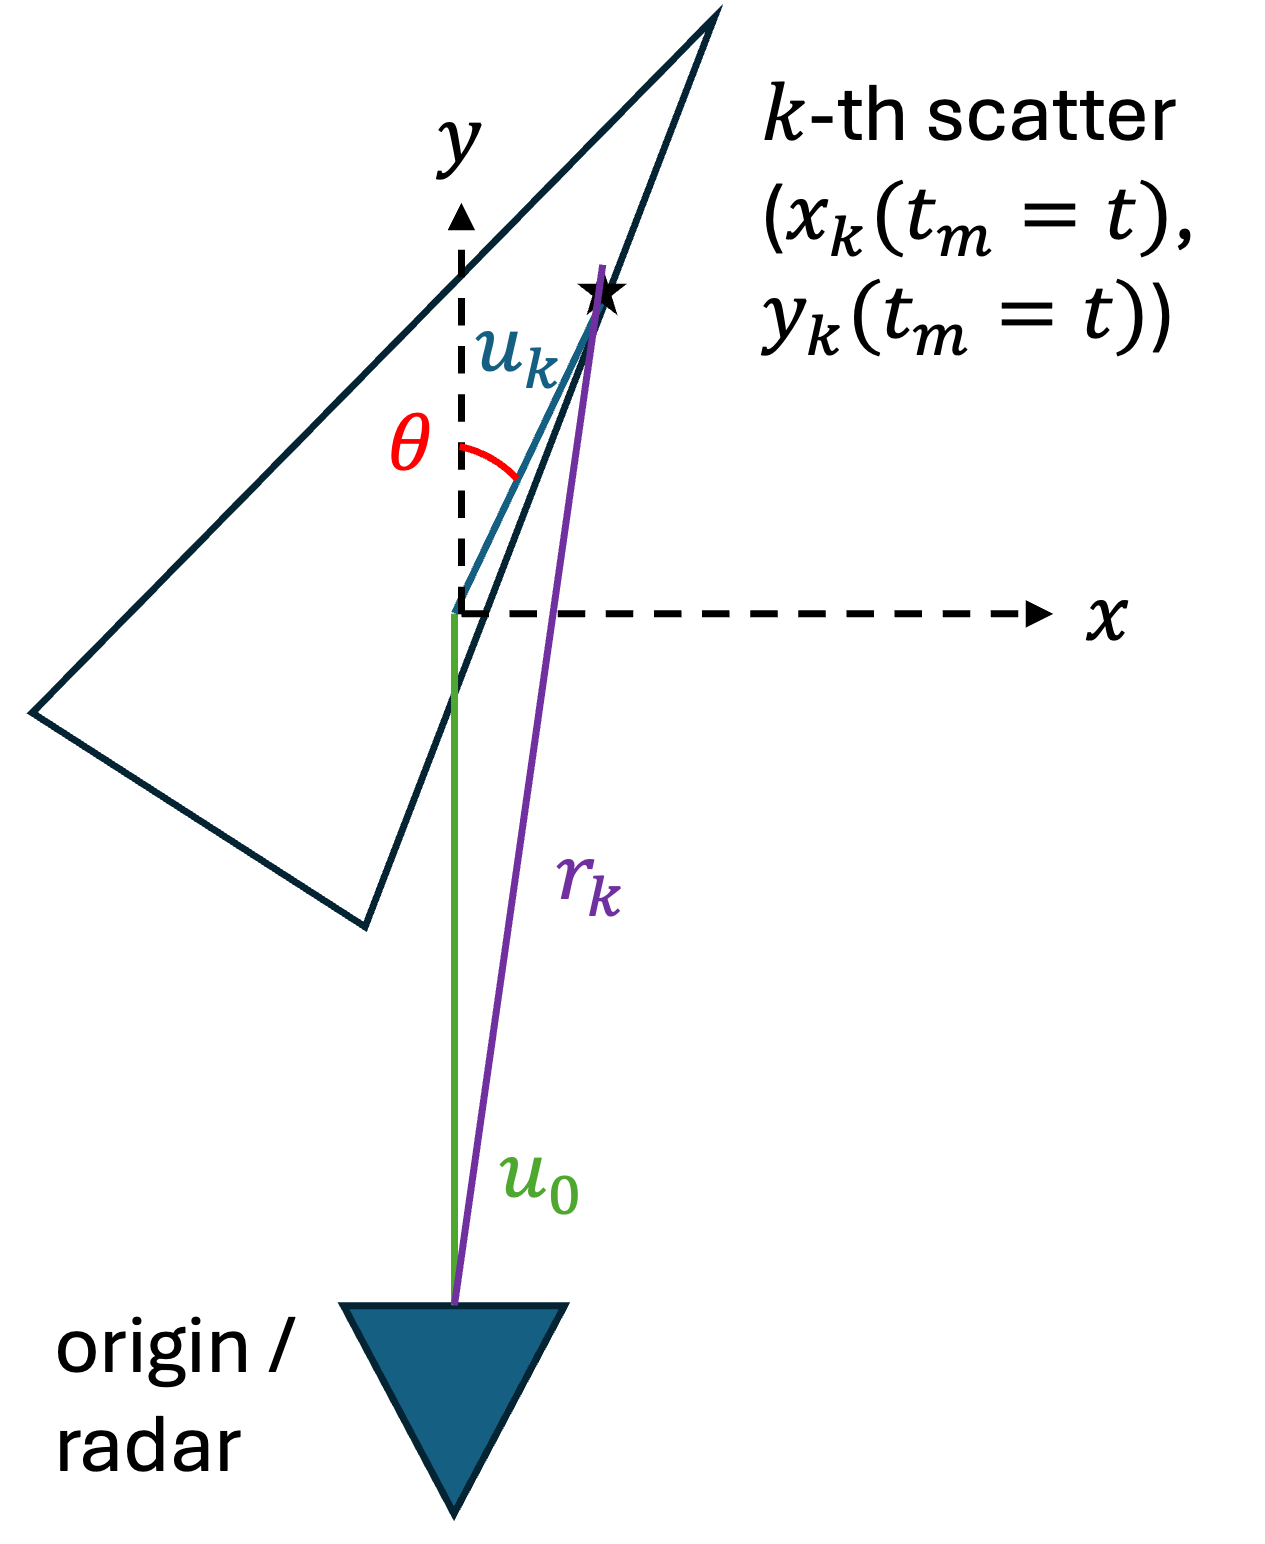
\includegraphics[width=0.5\linewidth]{figures/isar_geo2.png}
  \caption{ISAR target geometry as a function of slow-time}
  \label{fig:geo}
\end{figure}

\noindent The relative position of a scattering point as a function of slow-time ($t_{m}$) can be defined as \cite{Xu2022}:

\begin{equation}
    \begin{bmatrix}
        x_{k}(t_m)\\
        y_k (t_m)
    \end{bmatrix}
    =
    \begin{bmatrix}
        \cos(\theta(t_m)) & -\sin(\theta(t_{m})) \\
        \sin(\theta(t_m)) & \cos(\theta(t_m))
    \end{bmatrix}
    \begin{bmatrix}
        x_{k}\\
        y_k
    \end{bmatrix}
\end{equation}

\noindent where $\theta(t_{m})$ or $\theta_m$ is the angle of the target scatterer relative to the $y$-axis, and $[x_{k}, y_{k}]^{T}$ is the initial position of the $k$-th scatterer relative to the center of the rotation of the target. The range from the origin located at the radar to a scattering point is \cite{Xu2022}:
\begin{equation}
    \begin{aligned}
        r_{k}(t_m) &= \sqrt{x_{k}^2(t_m) + (y_k(t_{m}) + u_{0})^2}\\
        &\approx u_{0} + y_{k}(t_m) \quad \mathrm{as} \quad (y_k(t_{m}) + u_{0})^2 >> x_{k}^2(t_m)\\
        &= u_{0} + x_{k} \sin(\theta(t_{m})) + y_{k}\cos(\theta(t_{m}))\\
        &= u_{0} + u_{k} \\ &\mathrm{where} \quad u_{k} = x_{k} \sin(\theta(t_{m})) + y_{k}\cos(\theta(t_{m}))
    \end{aligned} 
    \label{eq:r}
\end{equation}

\noindent The angle $\theta_m$ can be approximated using a Taylor series:

\begin{equation}
    \begin{aligned}
        \sin(\theta) &= \theta - \frac{\theta^3}{3!} + \frac{\theta^{5}}{5!} + \dots \\
        \cos(\theta) &= 1 - \frac{\theta^2}{2!} + \frac{\theta^{4}}{4!} + \dots
    \end{aligned}
\end{equation}

\noindent For most ISAR applications, the target's rotation is relatively small across the coherent integration time, enabling the usage of the small angle approximation: $\sin(\theta(t_{m})) \approx\theta(t_{m})$ and $\cos(\theta(t_m)) \approx 1$. The range from the radar to a target scatterer can be approximated as:

\begin{equation}
  \begin{aligned}
    r_{k}(t_{m}) &\approx u_{0} + y_{k} + x_{k}\theta_{m} \\ \theta(t_{m}) &= \theta(0) + \omega t_{m} + \frac{\dot{\omega}}{2}t_{m}^{2} + \dots
  \end{aligned}
  \label{eq:r_final}
\end{equation}

% %%%%%%%%%%%%%%%%%%%%%%%%%%%%%%%%%%%%%%%%%%%%%%%%%%%%%%%%%%%%%%%%%%%%%%%%%%%%%%%%%%%%%%%%%%%%%%%%%%
% --------------------------------------------------------------------------------------------------
% %%%%%%%%%%%%%%%%%%%%%%%%%%%%%%%%%%%%%%%%%%%%%%%%%%%%%%%%%%%%%%%%%%%%%%%%%%%%%%%%%%%%%%%%%%%%%%%%%%
\subsection{Signal Model and Sensing Matrix} \label{sec:signal} 
% %%%%%%%%%%%%%%%%%%%%%%%%%%%%%%%%%%%%%%%%%%%%%%%%%%%%%%%%%%%%%%%%%%%%%%%%%%%%%%%%%%%%%%%%%%%%%%%%%%
% --------------------------------------------------------------------------------------------------
% %%%%%%%%%%%%%%%%%%%%%%%%%%%%%%%%%%%%%%%%%%%%%%%%%%%%%%%%%%%%%%%%%%%%%%%%%%%%%%%%%%%%%%%%%%%%%%%%%%

% target geometry
 The signal can be represented as a range-compressed echo:

\begin{equation}
    s(\hat{t},t_{m}) = C \cdot \text{sinc}(B(\hat{t} - \tau(t_{m})))\cdot \exp(-j2 \pi f_{c} \tau(t_{m}))
\end{equation}

\noindent where $C$ is the amplitude, $B$ is the bandwidth, $\hat{t}$ is the fast-time, $t_{m}$ is the slow-time, $\tau$ is the propagation delay and $f_{c}$ is the center frequency. The propagation delay for a monostatic radar configuration is the amount of time required to propagate to the target and return:

\begin{equation}
    \tau_{m} = \frac{2r(t_{m})}{c}
\end{equation}

\noindent where $r(t_{m})$ is the range or distance from the radar to a target scattering point as defined by equation \ref{eq:r}. The return echo can be represented as a summation of the returns from each scatterer:

\begin{equation}
    s(\hat{t},t_{m}) = C \sum_{k} \sigma_{k} \cdot \delta(\hat{t} - \tau_{k}(t_{m})) \cdot \exp(-j2 \pi f_{c} \tau_{k}(t_{m}))
\end{equation}

\noindent where $k$ is the index of each scatterer located at $\delta(\hat{t} - \tau_{k}(t_{m}))$, $K$ is the total number of scatterers or sparsity, and $\sigma_{k}$ is the complex reflectivity of the $k$-th scatterer. Typical formulations will assume separability in the range and crossrange to simplify the sensing matrix's formulation; however, this approach neglects the cross-terms inherent to range-cell migration. To preserve this effect while still defining a linear system suitable for reconstruction using compressed sensing, apply the Fourier transform in the fast-time:

\begin{equation}
    S(\hat{f},t_{m}) = C \sum_{k} \sigma_{k} \cdot \exp(-j2 \pi (f_{c} + \hat{f}) \tau_{k}(t_{m}))
    \label{eq:S}
\end{equation}

\noindent where $\hat{f}$ is the temporal-frequency or the range-frequency. Equation \ref{eq:S} enables a formulation of a sensing matrix where each entry can be defined as:

\begin{equation}
    A[{m + \ell M}, k] = C \sigma_{k} \cdot \exp(-j2 \pi (f_{c} + \hat{f}_{\ell}) \tau_{k}(t_{m}))
\end{equation}

\noindent The resulting linear system is defined as: $y = Ax + n$, where $y \in \mathbb{C}^{ML}$ is the measurement, $A \in \mathbb{C}^{ML \times K}$ is the sensing matrix, and $x \in \mathbb{C}^{K}$ is the vectorized latent image. The dimensionality of the system is determined by the number of range-frequency samples $L$, the number of scatterers $K$ and the number of received pulses $M$ which is less than the number of total pulses $N$ such that $M << N$. Figure \ref{fig:sensing_matrix} depicts the dimensionality of the proposed sensing matrix. 

\begin{figure}[h]
  \centering
  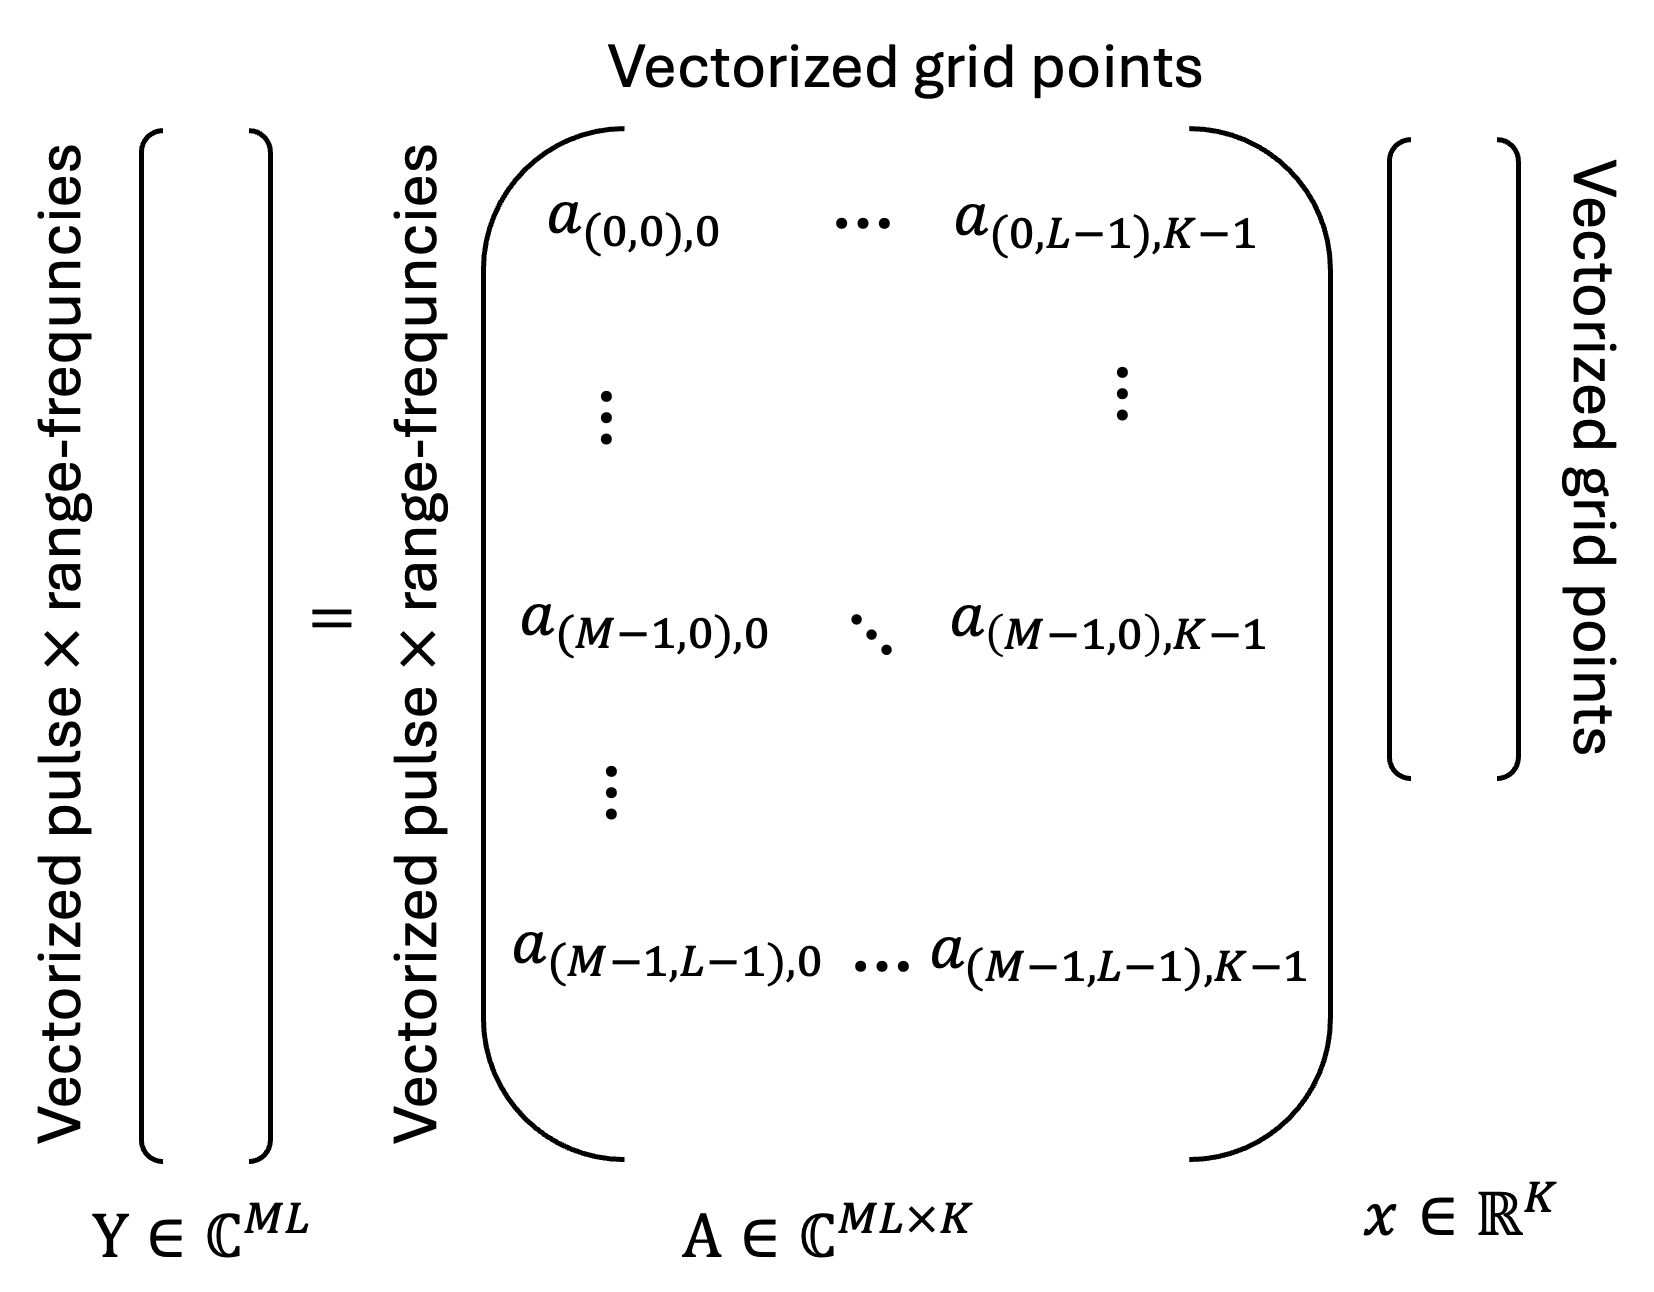
\includegraphics[width=0.75\linewidth]{figures/linear_sys1.png}
  \caption{Linear system formulation and dimensionality}
  \label{fig:sensing_matrix}
\end{figure}

This system is underdetermined and has infinitely many solutions, each existing in the ($N-M$)-dimensional null space of the sensing matrix. However, to treat this as a compressed sensing problem, if the latent image can be assumed $K$-sparse or containing $K$ non-zero values, the problem becomes $K$-dimensional where $M \geq K$. Additionally, if the sensing matrix is roughly orthogonal and incoherent, associated with the Restricted Isometric Property (RIP), the solution can be unique \cite{Majumdar_2018}. The compressed sensing problem can then be formulated as:

\begin{equation}
    \min_{x} ||x||_{0} \quad \text{subject to} \quad y = Ax
    \label{eq:l0}
\end{equation}

There are many different compressed sensing techniques, and Greedy algorithms like Orthogonal Matching Pursuit (OMP) are effective for non-linear recovery \cite{Bostock_2017}. For a Hermitian sensing matrix ($A$) where $A^{-1} = A^{H}$, OMP iterates through a defined sparsity ($K$) and finds the indices ($\Lambda$) that maximize the projection of the residual, initialized as the measurement, onto the basis vectors formed by $A$. The maximization of the residual selects the coefficients projected on the basis vectors formed by $A$, and the step $r = y - A \hat{X}$ prevents the re-selection of the same indices. The latent image estimation $\hat{X}$ is the least-squares approximation formed from the selected basis vectors of $A$. Algorithm \ref{algo:OMP} formally describes the OMP algorithm \cite{Majumdar_2018}.

\begin{algorithm}[H]
\caption{Orthogonal Matching Pursuit}\label{algo:OMP}
\begin{algorithmic}[1]
\Procedure{OMP}{$H,N$}
\State $\Lambda\gets []$
\State $r \gets y$
\State $\hat{X} \gets 0$
\For{$i \leq K$}
\State $c\gets A^{H}r$
\State $\Lambda = \arg\max_{i} \big| c_i \big|$
\State $\Lambda \gets \begin{bmatrix} \Lambda \\ l \end{bmatrix}$
\State $\hat{X} \gets (A(\Lambda)^{H}A(\Lambda))^{-1}A(\Lambda)^{H}y$
\State $r \gets y - A\hat{X}$
\State $i \gets i + 1$
\EndFor
\State \textbf{return} $\hat{X}$
\EndProcedure
\end{algorithmic}
\end{algorithm}

% %%%%%%%%%%%%%%%%%%%%%%%%%%%%%%%%%%%%%%%%%%%%%%%%%%%%%%%%%%%%%%%%%%%%%%%%%%%%%%%%%%%%%%%%%%%%%%%%%%
% --------------------------------------------------------------------------------------------------
% %%%%%%%%%%%%%%%%%%%%%%%%%%%%%%%%%%%%%%%%%%%%%%%%%%%%%%%%%%%%%%%%%%%%%%%%%%%%%%%%%%%%%%%%%%%%%%%%%%
\section{Modified OMP}
% %%%%%%%%%%%%%%%%%%%%%%%%%%%%%%%%%%%%%%%%%%%%%%%%%%%%%%%%%%%%%%%%%%%%%%%%%%%%%%%%%%%%%%%%%%%%%%%%%%
% --------------------------------------------------------------------------------------------------
% %%%%%%%%%%%%%%%%%%%%%%%%%%%%%%%%%%%%%%%%%%%%%%%%%%%%%%%%%%%%%%%%%%%%%%%%%%%%%%%%%%%%%%%%%%%%%%%%%%


% %%%%%%%%%%%%%%%%%%%%%%%%%%%%%%%%%%%%%%%%%%%%%%%%%%%%%%%%%%%%%%%%%%%%%%%%%%%%%%%%%%%%%%%%%%%%%%%%%%
% --------------------------------------------------------------------------------------------------
% %%%%%%%%%%%%%%%%%%%%%%%%%%%%%%%%%%%%%%%%%%%%%%%%%%%%%%%%%%%%%%%%%%%%%%%%%%%%%%%%%%%%%%%%%%%%%%%%%%
\section{Results}
% %%%%%%%%%%%%%%%%%%%%%%%%%%%%%%%%%%%%%%%%%%%%%%%%%%%%%%%%%%%%%%%%%%%%%%%%%%%%%%%%%%%%%%%%%%%%%%%%%%
% --------------------------------------------------------------------------------------------------
% %%%%%%%%%%%%%%%%%%%%%%%%%%%%%%%%%%%%%%%%%%%%%%%%%%%%%%%%%%%%%%%%%%%%%%%%%%%%%%%%%%%%%%%%%%%%%%%%%%


% %%%%%%%%%%%%%%%%%%%%%%%%%%%%%%%%%%%%%%%%%%%%%%%%%%%%%%%%%%%%%%%%%%%%%%%%%%%%%%%%%%%%%%%%%%%%%%%%%%
% --------------------------------------------------------------------------------------------------
% %%%%%%%%%%%%%%%%%%%%%%%%%%%%%%%%%%%%%%%%%%%%%%%%%%%%%%%%%%%%%%%%%%%%%%%%%%%%%%%%%%%%%%%%%%%%%%%%%%
\section{Discussion}
% %%%%%%%%%%%%%%%%%%%%%%%%%%%%%%%%%%%%%%%%%%%%%%%%%%%%%%%%%%%%%%%%%%%%%%%%%%%%%%%%%%%%%%%%%%%%%%%%%%
% --------------------------------------------------------------------------------------------------
% %%%%%%%%%%%%%%%%%%%%%%%%%%%%%%%%%%%%%%%%%%%%%%%%%%%%%%%%%%%%%%%%%%%%%%%%%%%%%%%%%%%%%%%%%%%%%%%%%%


% %%%%%%%%%%%%%%%%%%%%%%%%%%%%%%%%%%%%%%%%%%%%%%%%%%%%%%%%%%%%%%%%%%%%%%%%%%%%%%%%%%%%%%%%%%%%%%%%%%
% --------------------------------------------------------------------------------------------------
% %%%%%%%%%%%%%%%%%%%%%%%%%%%%%%%%%%%%%%%%%%%%%%%%%%%%%%%%%%%%%%%%%%%%%%%%%%%%%%%%%%%%%%%%%%%%%%%%%%
\section{Conclusion}
% %%%%%%%%%%%%%%%%%%%%%%%%%%%%%%%%%%%%%%%%%%%%%%%%%%%%%%%%%%%%%%%%%%%%%%%%%%%%%%%%%%%%%%%%%%%%%%%%%%
% --------------------------------------------------------------------------------------------------
% %%%%%%%%%%%%%%%%%%%%%%%%%%%%%%%%%%%%%%%%%%%%%%%%%%%%%%%%%%%%%%%%%%%%%%%%%%%%%%%%%%%%%%%%%%%%%%%%%%


\appendices
\section{Proof of the First Zonklar Equation}
Appendix one text goes here.

% you can choose not to have a title for an appendix
% if you want by leaving the argument blank
\section{}
Appendix two text goes here.


% use section* for acknowledgment
\section*{Acknowledgment}


The authors would like to thank...


% Can use something like this to put references on a page
% by themselves when using endfloat and the captionsoff option.
\ifCLASSOPTIONcaptionsoff
  \newpage
\fi

\printbibliography

\begin{IEEEbiography}{Michael Shell}
Biography text here.
\end{IEEEbiography}

% if you will not have a photo at all:
\begin{IEEEbiographynophoto}{John Doe}
Biography text here.
\end{IEEEbiographynophoto}

% insert where needed to balance the two columns on the last page with
% biographies
%\newpage

\begin{IEEEbiographynophoto}{Jane Doe}
Biography text here.
\end{IEEEbiographynophoto}

% You can push biographies down or up by placing
% a \vfill before or after them. The appropriate
% use of \vfill depends on what kind of text is
% on the last page and whether or not the columns
% are being equalized.

%\vfill

% Can be used to pull up biographies so that the bottom of the last one
% is flush with the other column.
%\enlargethispage{-5in}



% that's all folks
\end{document}
